\documentclass[tikz,border=4pt]{standalone}
\usepackage{amsmath,amssymb}
\usetikzlibrary{arrows.meta,calc,decorations.pathreplacing}
\definecolor{cA}{HTML}{924800}
\definecolor{cB}{HTML}{2F7FC8}
\definecolor{cC}{HTML}{39994B}
\tikzset{
  pt/.style={circle,fill=black,inner sep=0pt,minimum size=4pt},
  disp/.style={-{Stealth[length=2.6mm,width=2mm]},line width=0.9pt,shorten <=2.5pt,shorten >=2.5pt},
  lab/.style={font=\small,sloped,text=black},
  brc/.style={decorate,decoration={brace,amplitude=5pt,raise=3pt},line width=0.6pt},
}
\begin{document}
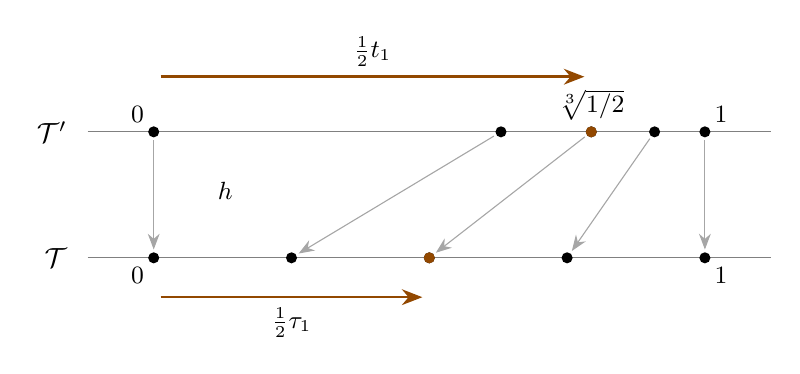
\begin{tikzpicture}[x=7cm]
  \draw[gray] (-0.12,1.6) -- (1.12,1.6); \draw[gray] (-0.12,0) -- (1.12,0);
  \node[anchor=east] at (-0.14,1.6) {$\mathcal{T}'$}; \node[anchor=east] at (-0.14,0) {$\mathcal{T}$};
  \foreach \k in {0,1,2,3,4}{
    \pgfmathsetmacro{\top}{(\k/4)^(1/3)}
    \draw[gray!70,-{Stealth[length=2mm]},shorten <=3pt,shorten >=3pt] (\top,1.6) -- (\k/4,0);
    \node[pt] at (\top,1.6) {}; \node[pt] at (\k/4,0) {};
  }
  \pgfmathsetmacro{\half}{0.5^(1/3)}
  \node[pt,fill=cA] at (\half,1.6) {}; \node[pt,fill=cA] at (0.5,0) {};
  \draw[disp,cA] (0,2.3) -- node[above,font=\small,text=black]{$\tfrac12 t_1$} (\half,2.3);
  \draw[disp,cA] (0,-0.5) -- node[below,font=\small,text=black]{$\tfrac12\tau_1$} (0.5,-0.5);
  \node[above,font=\small] at (\half,1.62) {$\sqrt[3]{1/2}$};
  \node[above left,font=\small] at (0,1.6) {$0$}; \node[above right,font=\small] at (1,1.6) {$1$};
  \node[below left,font=\small] at (0,0) {$0$}; \node[below right,font=\small] at (1,0) {$1$};
  \node[font=\small] at (0.13,0.85) {$h$};
\end{tikzpicture}
\end{document}
